\documentclass{article}
\usepackage[preprint]{neurips_2025}
\usepackage[utf8]{inputenc}
\usepackage[T1]{fontenc}
\usepackage[pagebackref,breaklinks,colorlinks,citecolor=blue,linkcolor=red]{hyperref}

\usepackage{url}
\usepackage{booktabs}
\usepackage{amsfonts}
\usepackage{amsmath}
\usepackage{nicefrac}
\usepackage{microtype}
\usepackage{booktabs}
\usepackage[table]{xcolor}
\usepackage{graphicx}
\usepackage{algorithm}
\usepackage{algorithmic}
\usepackage{multirow}
\usepackage{enumitem}
\usepackage{subcaption}
\usepackage{tikz}
\usepackage{comment}
\usepackage[capitalize,noabbrev]{cleveref}


\newcommand{\circled}[1]{\tikz[baseline=(char.base)]{
  \node[shape=circle,draw,inner sep=1pt] (char) {\small #1};}}



\newcommand{\todoc}[2]{{\textcolor{#1}{\textbf{#2}}}}
\newcommand{\todored}[1]{{\todoc{red}{\textbf{[#1]}}}}
\newcommand{\todogreen}[1]{\todoc{green}{\textbf{[#1]}}}
\newcommand{\todoblue}[1]{\todoc{blue}{\textbf{[#1]}}}
\newcommand{\todoorange}[1]{\todoc{orange}{\textbf{[#1]}}}
\newcommand{\todobrown}[1]{\todoc{brown}{\textbf{[#1]}}}
\newcommand{\todogray}[1]{\todoc{gray}{\textbf{[#1]}}}
\newcommand{\todopink}[1]{\todoc{pink}{\textbf{[#1]}}}
\newcommand{\todoyellow}[1]{\todoc{yellow}{\textbf{[#1]}}}
\newcommand{\todopurple}[1]{\todoc{purple}{\textbf{[#1]}}}



\newcommand{\txhan}[1]{\todoblue{txhan: #1}}

\newcommand{\wei}[1]{\textcolor{orange}{#1}}

\title{\ours{}: Do Agent Skills Actually Help in Real-World Software Engineering?}
\author{
  Tingxu Han \footnotemark[1]\\
  Nanjing University \\
  Mohamed bin Zayed University of Artificial Intelligence \\
  \texttt{txhan@smail.nju.edu.cn} \\[-0.3em]
  \And
  Yi Zhang \\
  South China University of Technology \\
  \texttt{202330580551@mail.scut.edu.cn} \\[-0.3em]
  \And
  Wei Song \\
  The University of New South Wales \\
  \texttt{wei.song1@unsw.edu.au} \\[-0.3em]
  \And
  Chunrong Fang \footnotemark[3]\\
  Nanjing University \\
  \texttt{fangchunrong@nju.edu.cn} \\[-0.3em]
  \And
  Zhenyu Chen \\
  Nanjing University \\
  \texttt{zychen@nju.edu.cn} \\[-0.3em]
  \And
  Youcheng Sun \\
  Mohamed bin Zayed University of Artificial Intelligence \\
  \texttt{youcheng.sun@mbzuai.ac.ae} \\[-0.3em]
  \And
  Lijie Hu \footnotemark[3]\\
  Mohamed bin Zayed University of Artificial Intelligence \\
  \texttt{lijie.hu@mbzuai.ac.ae} \\
}
\newcommand{\ours}{SWE-Skills-Bench}

\renewcommand*\sectionautorefname{Section}
\def\sectionautorefname{Section}
\def\subsectionautorefname{Section}
\def\subsubsectionautorefname{Section}
\def\subfigureautorefname{Figure}

\begin{document}
\maketitle
\renewcommand{\thefootnote}{\fnsymbol{footnote}}
\footnotetext[1]{Work done during a research visit at MBZUAI.}
\footnotetext[3]{Corresponding Author.}
\footnotetext{Pre-print with preliminary results, work in progress.}
\vspace{-2em}
\begin{abstract}
Agent skills, structured procedural knowledge packages injected at inference time, are increasingly used to augment LLM agents on software engineering tasks.
However, their real utility in end-to-end development settings remains unclear.
We present \textbf{\ours{}}, the first requirement-driven benchmark that isolates the marginal utility of agent skills in real-world software engineering (SWE).
It pairs 49 public SWE skills with authentic GitHub repositories pinned at fixed commits and requirement documents with explicit acceptance criteria, yielding approximately 565 task instances across six SWE subdomains.
We introduce a deterministic verification framework that maps each task's acceptance criteria to execution-based tests, enabling controlled paired evaluation with and without the skill.
Our results show that skill injection benefits are far more limited than rapid adoption suggests: 39 of 49 skills yield zero pass-rate improvement, and the average gain is only $+1.2\%$. Token overhead varies from modest savings to a $451\%$ increase while pass rates remain unchanged. Only seven specialized skills produce meaningful gains (up to $+30\%$), while three degrade performance (up to $-10\%$) due to version-mismatched guidance conflicting with project context.
These findings suggest that agent skills are a narrow intervention whose utility depends strongly on domain fit, abstraction level, and contextual compatibility.
SWE-Skills-Bench provides a testbed for evaluating the design, selection, and deployment of skills in software engineering agents.
\ours{} is available at \url{https://github.com/GeniusHTX/SWE-Skills-Bench}.
\begin{comment}
Agent skills, structured procedural knowledge packages injected at inference time, are increasingly used to augment LLM agents on software engineering tasks. However, their real utility in end-to-end development settings remains unclear.
We present \textbf{\ours{}}, the first requirement-driven benchmark that isolates the marginal utility of agent skills in real-world software engineering (SWE).
It contains
49 public SWE skills, each
paired with an authentic GitHub 
repositories pinned
at a fixed commits and requirement documents with explicit acceptance criteria, yielding approximately 565 task instances across eight SWE subdomains, including DevOps, observability, ML engineering, financial modelling, security, data engineering, and backend frameworks. 
To assess whether a skill truly helps, we introduce a requirement-driven deterministic verification framework that maps each task's acceptance criteria to execution-based tests, enabling controlled paired evaluation with and without the skill. 
Our results show that the benefit of skill injection is far more limited than its rapid adoption suggests. 
Across all 49 skills, 39 yield zero pass-rate improvement, and the average gain is only $+1.2\%$.  Skill overhead varies dramatically,  from modest token savings to a $451\%$ increase in token usage, while pass rates often remain unchanged. Only a small subset of seven specialized skills, such as those encoding financial risk formulas, produces meaningful gains ($+30\%$), while three skills degrade performance ($-10\%$) because version-mismatched guidance conflicts with the project context.
These findings suggest that agent skills are not a universal performance booster for SWE agents, but a narrow intervention whose utility depends strongly on domain fit, abstraction level, and contextual compatibility. SWE-Skills-Bench offers a testbed for evaluating skill design, selection, and deployment in software engineering agents.
\ours{} is available at \url{https://github.com/GeniusHTX/SWE-Skills-Bench}.
\end{comment}
\end{abstract}
\section{Introduction}
\label{sec:intro}

\begin{figure}[t]
    \centering
  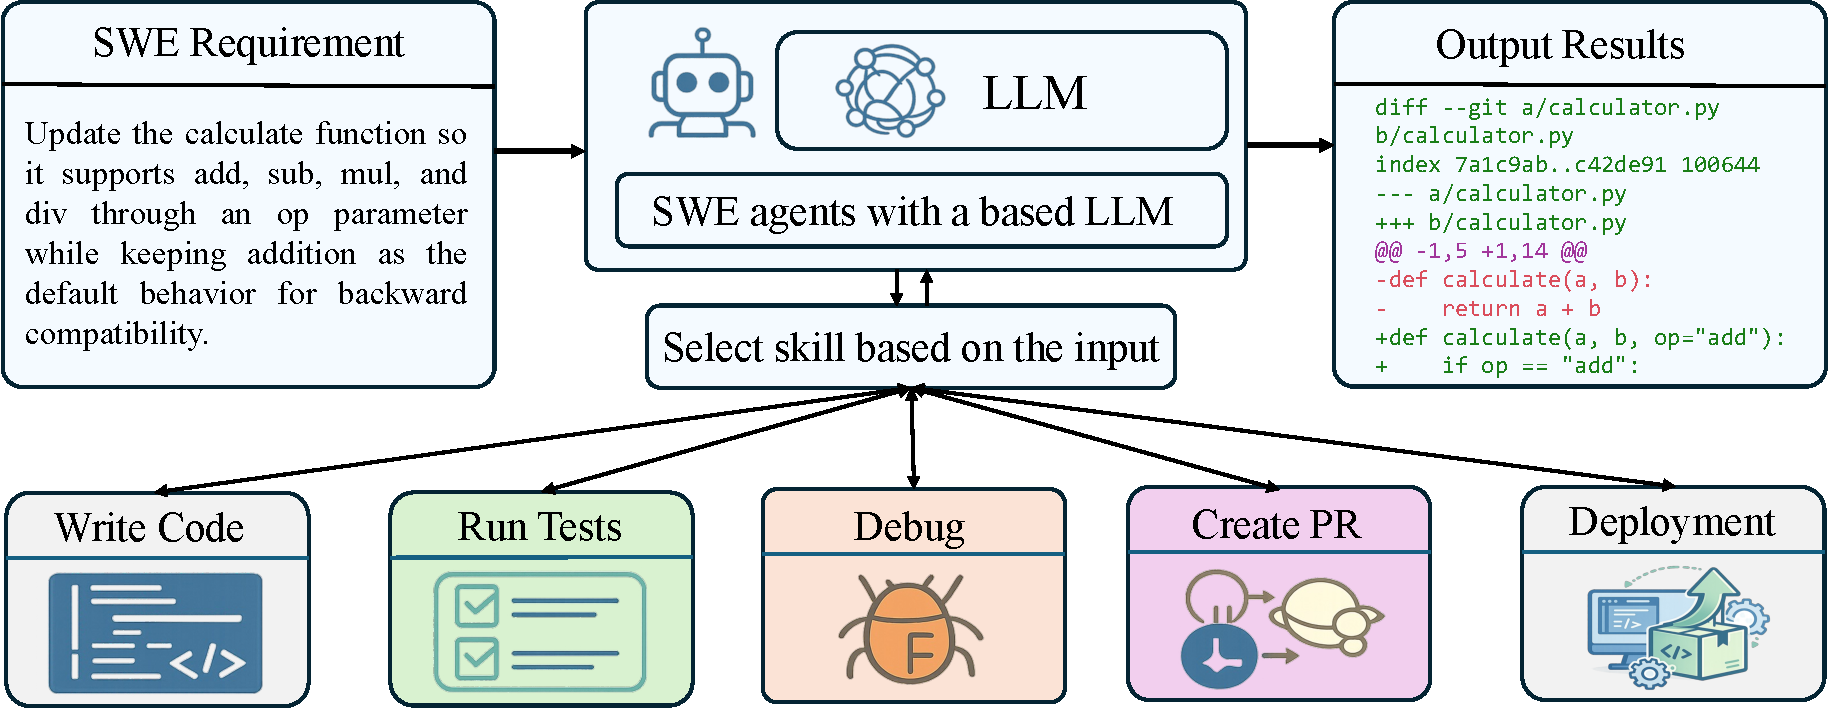
\includegraphics[width=0.98\columnwidth]{Figures/skills-example.pdf}
  \caption{Illustration of how agent skills are used in a software engineering workflow. Given a natural-language requirement, the LLM-based agent selects the most relevant skill from its skill library, including skills such as writing code, running tests, debugging, creating pull requests, and deploying, and injects it into the context window. The agent then executes a series of SWE actions to produce the final software artifacts (such as code) that fulfill the requirement.}
\label{fig:skill-augmentation}
\end{figure}

LLM-based agents have been increasingly deployed across a wide range of software engineering (SWE) tasks, from automated code generation and bug fixing~\cite{jimenez2024swebench} to CI/CD pipeline configuration and infrastructure management~\cite{yang2024sweagent,song2025help}. 
Agent Skills are structured markdown packages that encode procedural knowledge,standard operating procedures, code templates, and domain conventions,for consumption by LLM-based agents~\cite{anthropic2025skills,fang2025memp,wang2023voyager,wang2024survey,xu2026agentskills}. 
At inference time, a skill is simply injected into the agent's context window as a reference document.
Unlike fine-tuning or retrieval-augmented generation, no model modification or external retrieval pipeline is required (\autoref{fig:skill-augmentation} illustrates how agent skills work given a software engineering task). 
The ecosystem has grown explosively: over 84{,}192 skills were created in just 136 days~\cite{li2026skillsbench}. 

Despite this rapid adoption, no existing benchmark evaluates SWE skills in real-world software development scenarios. 
TerminalBench~\cite{merrill2026terminalbench} evaluates CLI tasks in multi-file repositories, but does not include a skill-augmentation condition.
HumanEval~\cite{chen2021humaneval} and BigCodeBench~\cite{zhuo2025bigcodebench} target self-contained function completion without multi-file context or skill augmentation. 
SkillsBench~\cite{li2026skillsbench} is the first cross-domain benchmark to evaluate agent skills as first-class artifacts under paired skill conditions and deterministic verification. However, it is not specifically designed for software engineering: SWE constitutes only 16 of its 84 tasks, and its primary goal is to measure broad cross-domain skill efficacy rather than requirement satisfaction in real-world development workflows.

A principled benchmark for SWE skill utility must answer a deceptively simple question: \emph{Does the skill help the agent satisfy the task's requirements?}
Software engineering is inherently requirement-driven~\cite{sommerville2015software,zave1997classification,pohl2010requirements}: a task succeeds when every acceptance criterion stated in its specification is met, and unit tests serve as the executable encoding of those criteria.
We therefore adopt a \textbf{requirement-driven evaluation} methodology: each task is anchored to a requirement document that defines scope and acceptance criteria, and deterministic verifiers based on unit tests are systematically derived from those criteria, establishing full traceability from requirements to test verdicts.

Building on this methodology, we present \textbf{\ours{}}, a benchmark designed to isolate the marginal utility of agent skills for software engineering. 
We curate 49 SWE skills from public repositories, pair each with an authentic GitHub project pinned at a fixed commit, and evaluate under controlled with-skill vs.\ without-skill conditions. 
All task instances are verified by deterministic, execution-based checks with no reliance on LLM-as-judge evaluation.

Our main contributions are as follows:
\begin{itemize}[leftmargin=*]
    \item \textbf{Benchmark.} We build \ours{}, a benchmark of 49 real-world SWE skills with ${\sim}11$ task instances per skill (${\sim}565$ total). Tasks are sourced from public skill repositories and evaluated on fixed-commit GitHub projects in containerized environments.
    \item \textbf{Requirement-driven test harness.} We design an automated unit-testing mechanism that translates each SWE requirement into executable test cases, deterministically verifying whether the specified requirement is fulfilled under both with-skill and without-skill conditions.
    \item \textbf{Empirical findings.}\circled{1}~Skill injection yields limited marginal gains: 39 of 49 skills produce $\Delta_P = 0$, and the average pass-rate improvement is a modest $+1.2\%$.
\circled{2}~Token overhead is decoupled from correctness: even among skills with zero delta, the token overhead ratio $\rho$ ranges from $-78\%$ to $+451\%$, indicating that skills reshape the agent's reasoning path without necessarily improving outcomes.
\circled{3}~A small subset of 7 skills encoding specialized procedural knowledge---financial risk formulas, cloud-native traffic management, and GitLab CI patterns---delivers meaningful gains up to $+30\%$.
\circled{4}~Three skills produce negative deltas (up to $-10\%$) when their version-specific conventions conflict with the target project's framework, demonstrating that skill injection carries a structural risk of context interference.
These results establish that SWE skill utility is highly domain-specific and context-dependent, favoring targeted skill design over blanket adoption.
\end{itemize}
\section{Related Benchmarks \& Datasets}
\label{sec:related}

We organize related work into two threads: SWE- and Skill-related benchmarks.
Generally, SWE-related benchmarks does not include skills in their evaluation, Skill-related benchmarks does focus on SWE tasks.
To the best of our knowledge, we are the first benchmark to evaluate agent skills in software engineering.
\autoref{tab:comparison} summarizes the key differences.

\textbf{SWE-related Benchmarks.}
This line of work can be further divided into SWE real-world benchmarks and code generation benchmarks.
SWE real-world benchmarks focus on realistic, project-level software engineering tasks with execution-based verification.
SWE-Bench Verified~\cite{jimenez2024swebench} is a human-validated subset of 500 instances from SWE-Bench, drawn from 12 Python repositories and evaluated via fail-to-pass tests.
TerminalBench~\cite{merrill2026terminalbench} evaluates agents on 200 realistic CLI tasks in containerized environments and provides methodological inspiration for our evaluation setup. However, these benchmarks do not isolate the marginal benefit of injecting procedural skill documents.
Code generation benchmarks, in contrast, mainly evaluate models on self-contained coding problems (often algorithmic or snippet-level) without full project context. HumanEval~\cite{chen2021humaneval} comprises 164 hand-crafted programming challenges at the function level, and therefore does not capture multi-file reasoning, dependency management, or end-to-end SWE workflows.

\textbf{Skills Benchmarks.}
SkillsBench~\cite{li2026skillsbench} takes an important first step toward benchmarking skills as first-class artifacts by comparing agent performance across different skill conditions. Nevertheless, it is not SWE-specific: software engineering forms only a limited subset of its task suite, and the benchmark is not designed around the central success criterion in real-world development—whether explicit requirements are satisfied in repository-grounded workflows. Our work addresses this gap by constructing a requirement-driven benchmark focused exclusively on SWE, where each skill is paired with fixed-commit repositories, explicit requirements, and deterministic execution-based verification.

\begin{comment}
SkillsBench~\cite{li2026skillsbench} is an early benchmark that treats skills as first-class artifacts and evaluates performance under different skill conditions (e.g., no-skill vs. skill-augmented). However, it is not specifically designed for software engineering: SWE constitutes only 16 of its 84 tasks, and its primary goal is to measure broad cross-domain skill efficacy rather than requirement satisfaction in real-world development workflows.
\end{comment}

\begin{table}[t]
\centering
\caption{Comparison of \ours{} with existing benchmarks. ``Skill Cond.'' indicates whether the benchmark includes agent skills. ``Det. Verifier'' indicates whether deterministic (non-LLM) verification is included. ``SWE-Focused'' indicates whether the benchmark is specifically designed for software engineering tasks.}
\label{tab:comparison}
\small
\begin{tabular}{lccccc}
\toprule
\textbf{Benchmark} & \textbf{Size} & \textbf{Skill Cond.} & \textbf{Real Projects} & \textbf{Det. Verifier} & \textbf{SWE-Focused} \\
\cmidrule(lr){1-6}
SWE-Bench Verified \cite{jimenez2024swebench} & 500 & None & Yes & Yes & Yes \\
TerminalBench \cite{merrill2026terminalbench} & 200 & None & Yes & Yes & Yes \\
HumanEval \cite{chen2021humaneval} & 164 & None & No & Partial & No \\
SkillsBench \cite{li2026skillsbench} & 84 & Yes & Yes & Yes & Partial \\
\cmidrule(lr){1-6}
\textbf{\ours{}} & \textbf{565} & \textbf{Yes} & \textbf{Yes} & \textbf{Yes} & \textbf{Yes} \\
\bottomrule
\end{tabular}
\end{table}

\begin{figure}
    \centering
    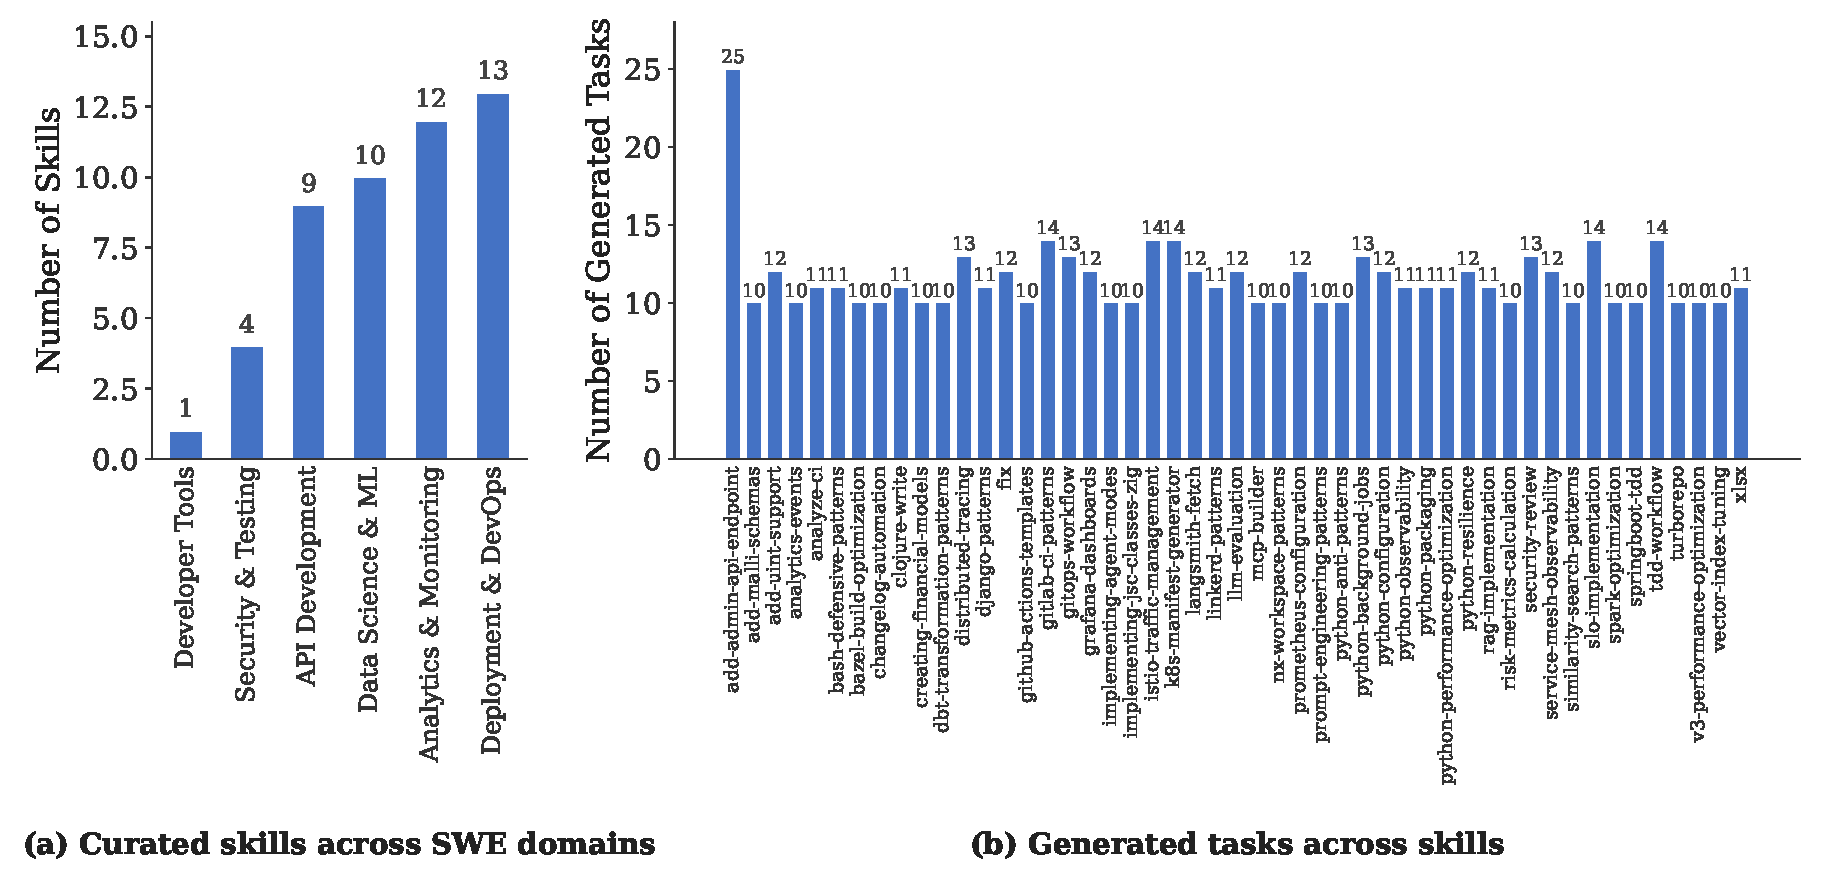
\includegraphics[width=0.99\linewidth]{Figures/fig_combined.pdf}
    \caption{The distribution of the curated skills and generated tasks.}
    \label{fig:distribution_skill_task}
\end{figure}


\begin{figure}
    \centering
    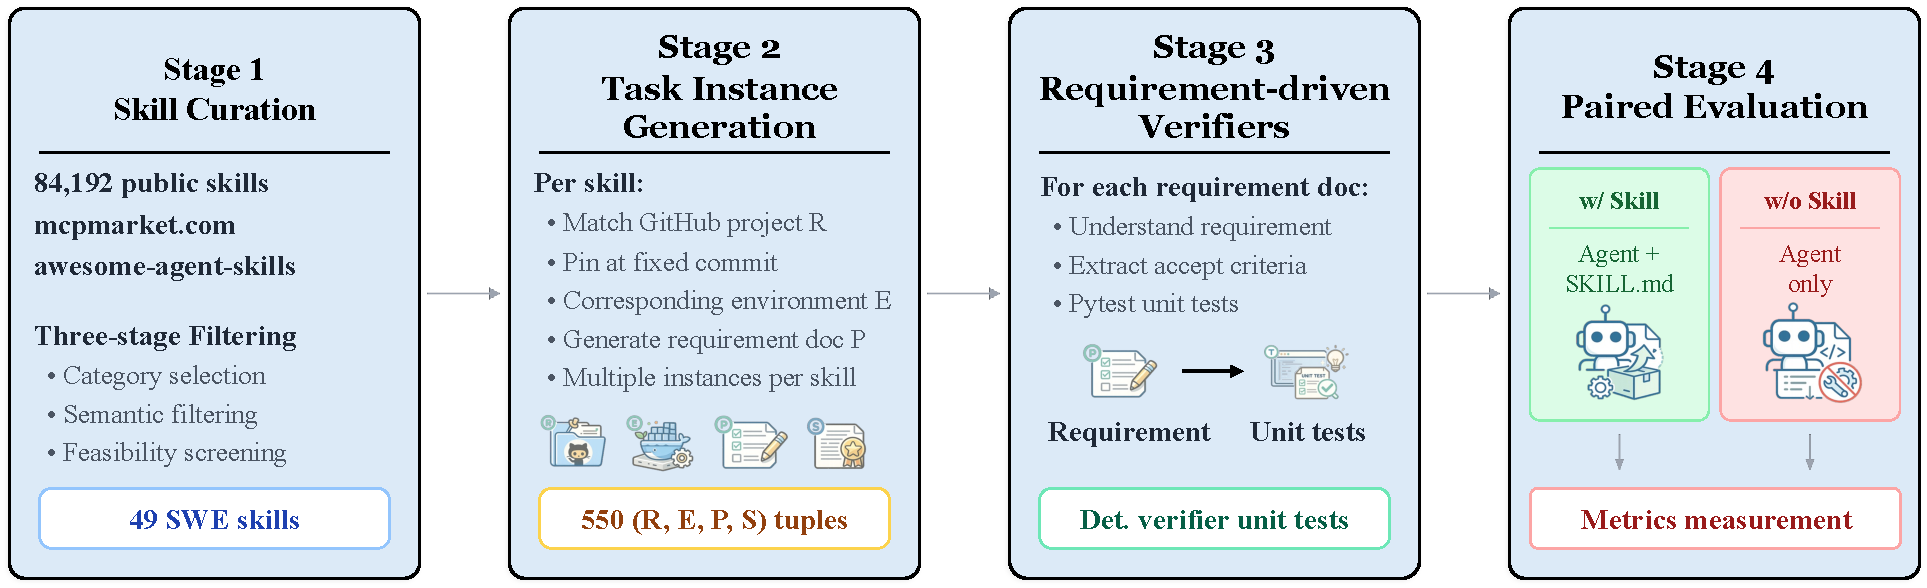
\includegraphics[width=0.98\linewidth]{Figures/bench-pipeline.pdf}
    \caption{Overview of the \ours{} construction pipeline. We begin with 84,192 public skills and narrow them down through three filtering stages: category selection, semantic filtering, and feasibility screening. This process yields 49 SWE skills (Stage 1). Next, for each skill, we identify a matching GitHub project and generate 565 task instances of the form $(R, E, P, S)$ (Stage 2). For each criterion in the requirements document $P$, we build deterministic verifiers using pytest unit tests (Stage 3). Finally, we run a paired evaluation that compares agent performance with and without the SKILL.md file, allowing us to measure the effectiveness of the skill (Stage 4).}
    \label{fig:pipeline}
\end{figure}

\section{\ours{} Construction}
\label{sec:data}
Constructing \ours{} requires answering three key questions in sequence: \emph{which} skills to benchmark, \emph{how} to pair each skill with authentic task instances, and \emph{how} to verify that the stated requirements are fulfilled. 
Our pipeline proceeds in four stages (\autoref{fig:pipeline}): (1) curating a representative set of SWE skills from large public repositories, (2) generating task instances by pairing each skill with a fixed-commit GitHub project and a requirement document, (3) designing deterministic verifiers that are traceable to the acceptance criteria in each requirement document.

\subsection{Skill Curation}
\label{subsec:curation}

The skill ecosystem is vast (84{,}192 skills created in 136 days~\cite{li2026skillsbench}) but highly heterogeneous in quality, scope, and evaluability. We curate a deterministic, unit-testable subset through a three-stage filtering pipeline. First, we scan the \texttt{mcpmarket} category leaderboard and select six of the nine core categories that best align with software-engineering workflows and are amenable to unit-test evaluation: Developer Tools, Security \& Testing, API Development, Data Science \& ML, Deployment \& DevOps, and Analytics \& Monitoring. Second, we apply semantic filtering to exclude generative or subjective skills, retaining only those that target concrete SWE actions such as \emph{fix}, \emph{build}, and \emph{develop}. Third, we exclude candidates whose associated repositories are prohibitively large or incur high environment and setup costs. This pipeline yields 49 skills distributed across the six categories: Deployment \& DevOps (13), Analytics \& Monitoring (12), API Development (10), Data Science \& ML (9), Security \& Testing (4), and Developer Tools (1). 
\autoref{fig:distribution_skill_task}(a) illustrates the distribution.
\begin{figure}[!h]
    \centering
    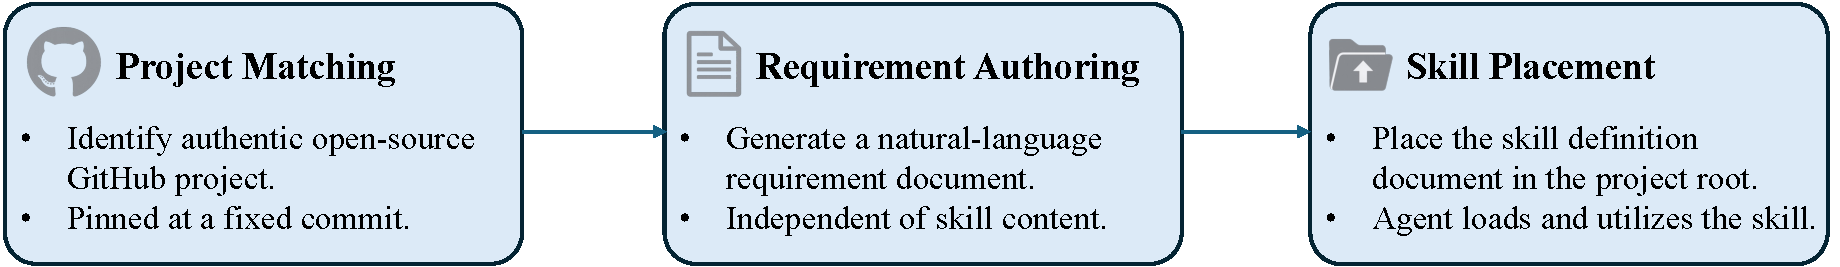
\includegraphics[width=0.99\linewidth]{Figures/task-instance-generation.pdf}
    \caption{The pipeline of task instance generation.}
    \label{fig:task-instance-gen}
\end{figure}




\subsection{Task Instance Generation}
\label{subsec:instance}

    As shown in \autoref{fig:task-instance-gen}, for each curated skill $s$, we construct approximately 10 task instances following a three-step procedure.
    
    \textbf{Project matching.} We identify an authentic, open-source GitHub project whose technology stack aligns with the skill's domain. The repository is pinned at a fixed commit to ensure reproducibility. Note that we also create a docker container for running each project.
    
    \textbf{Requirement authoring.} 
    Each requirement $P$ is authored to be specific to its target repository and skill-triggering conditions. To maximize structural clarity and eliminate ambiguity, every $P$ adheres to a standardized template comprising: (i) Background, providing the necessary task context; (ii) Requirement, defining the core objective; (iii) File Operations, specifying the files to be modified or created; and (iv) Acceptance Criteria, offering deterministic success metrics.
    \autoref{fig:requirement_gen_prompt} illustrates the prompt utilized to author the requirement and \autoref{fig:example_requirement} an example of the generated requirement.
    
    \textbf{Skill placement.} During the container preparation phase, the system removes the \texttt{.claude/skills} directory from the repository to eliminate interference from pre-existing skills. The activation of skill $S$ is governed by a file-level injection mechanism: the skill document $S$ is copied into the \texttt{\textasciitilde/.claude} directory only when the experimental condition requires its use; otherwise, it is omitted. The agent automatically detects and integrates any skills present in this environment. Importantly, the requirement document $P$ never references $S$, ensuring that the agent's behavior is governed strictly by the physical presence of the skill configuration.
        
Totally, for each skill, we generate around 10 instances where detailed distributions in \autoref{fig:distribution_skill_task}(b).
\subsection{Requirement-driven Verification}
\label{subsec:verifier}

The core principle of \ours{} is \emph{requirement-driven verification}. Rather than relying on subjective judgments, we convert every acceptance criterion in the requirement document $P$ into objective, deterministic tests, ensuring that each test outcome is directly traceable to a specific requirement.
We provide $P$ (together with repository metadata such as repo path, language, and available test commands) to a fixed “professional test engineer” prompt template, which instructs the model to (i) enumerate testable behaviors from each acceptance criterion, (ii) instantiate representative and edge-case scenarios, and (iii) encode them into a deterministic \texttt{pytest} test file with strong discriminative power (i.e., tests must run the produced code and verify concrete outputs/structures rather than keyword-level heuristics). The prompt also enforces structural constraints such as a minimum number of test cases and per-test docstrings. 
The prompt template is shown in \autoref{fig:test_gen_prompt}.

Concretely, for each instance we create a container from a base image, clone the target repository into the container workspace, and complete environment setup. We then pass the task document (i.e., the requirement document $P$) through the above prompt template to drive test generation, and use the task document as the prompt to Claude Code for implementation.


\subsection{Task Formulation}
\label{subsec:task_form}

Each task instance is a tuple $(R, E, P, S)$: a GitHub repository $R$ pinned at a fixed commit and the corresponding containerized running environment, a natural-language requirement document $P$ that specifies tasks, and optionally a skill document $S$. The agent (claude code specifically) must produce code changes, configuration files, or execution artifacts that satisfy the requirements in $P$ given the code repository $R$ and environment $E$.

In our evaluation methodology, every acceptance criterion in the requirement document $P$ is mapped to deterministic verifier, establishing full traceability from requirements to test verdicts.
\section{Results of \ours{}}
\label{sec:experiments}

\begin{table*}[t]
\centering
\caption{Evaluation results across all 49 skills. $\text{Pass}^{+}$ and $\text{Pass}^{-}$ denote pass rates with and without skill injection, respectively. $\Delta P$ is the skill utility delta, $C^{+}$ and $C^{-}$ are average token costs, $\rho$ is the token overhead ratio, and $\mathrm{CE}$ is cost efficiency. Best viewed in color.}
\label{tab:results}
\resizebox{\textwidth}{!}{%
\begin{tabular}{l c r r r r r r r}
\toprule
\textbf{Skills} & $\#$\textbf{Tasks} & $\textbf{Pass}^{+}$ & $\textbf{Pass}^{-}$ & $\boldsymbol{\Delta P}$ & $\boldsymbol{C^{+}}$ & $\boldsymbol{C^{-}}$ & $\boldsymbol{\rho}$ & $\textbf{CE}$ \\
\midrule
  \texttt{add-uint-support} & 12 & 100.0\% & 100.0\% & 0.0\% & 880K & 414K & \cellcolor{red!10}+112.6\% & --- \\
  \texttt{analytics-events} & 10 & 100.0\% & 100.0\% & 0.0\% & 321K & 157K & \cellcolor{red!10}+104.6\% & --- \\
  \texttt{analyze-ci} & 11 & 100.0\% & 100.0\% & 0.0\% & 66K & 74K & \cellcolor{green!10}-10.6\% & --- \\
  \texttt{dbt-transformation-patterns} & 10 & 100.0\% & 100.0\% & 0.0\% & 422K & 208K & \cellcolor{red!10}+103.2\% & --- \\
  \texttt{gitops-workflow} & 13 & 100.0\% & 100.0\% & 0.0\% & 130K & 57K & \cellcolor{red!10}+127.1\% & --- \\
  \texttt{grafana-dashboards} & 12 & 100.0\% & 100.0\% & 0.0\% & 150K & 116K & \cellcolor{red!10}+29.3\% & --- \\
  \texttt{implementing-agent-modes} & 10 & 100.0\% & 100.0\% & 0.0\% & 342K & 655K & \cellcolor{green!10}-47.8\% & --- \\
  \texttt{k8s-manifest-generator} & 14 & 100.0\% & 100.0\% & 0.0\% & 98K & 51K & \cellcolor{red!10}+91.2\% & --- \\
  \texttt{langsmith-fetch} & 12 & 100.0\% & 100.0\% & 0.0\% & 102K & 97K & \cellcolor{red!10}+5.9\% & --- \\
  \texttt{llm-evaluation} & 12 & 100.0\% & 100.0\% & 0.0\% & 238K & 203K & \cellcolor{red!10}+17.6\% & --- \\
  \texttt{mcp-builder} & 10 & 100.0\% & 100.0\% & 0.0\% & 273K & 200K & \cellcolor{red!10}+36.1\% & --- \\
  \texttt{nx-workspace-patterns} & 10 & 100.0\% & 100.0\% & 0.0\% & 417K & 365K & \cellcolor{red!10}+14.5\% & --- \\
  \texttt{prometheus-configuration} & 12 & 100.0\% & 100.0\% & 0.0\% & 225K & 312K & \cellcolor{green!10}-27.8\% & --- \\
  \texttt{python-anti-patterns} & 10 & 100.0\% & 100.0\% & 0.0\% & 274K & 490K & \cellcolor{green!10}-44.1\% & --- \\
  \texttt{python-background-jobs} & 13 & 100.0\% & 100.0\% & 0.0\% & 839K & 249K & \cellcolor{red!10}+236.8\% & --- \\
  \texttt{python-observability} & 11 & 100.0\% & 100.0\% & 0.0\% & 271K & 105K & \cellcolor{red!10}+157.5\% & --- \\
  \texttt{python-packaging} & 11 & 100.0\% & 100.0\% & 0.0\% & 167K & 74K & \cellcolor{red!10}+123.9\% & --- \\
  \texttt{python-performance-optimization} & 11 & 100.0\% & 100.0\% & 0.0\% & 91K & 96K & \cellcolor{green!10}-5.1\% & --- \\
  \texttt{python-resilience} & 12 & 100.0\% & 100.0\% & 0.0\% & 119K & 529K & \cellcolor{green!10}-77.6\% & --- \\
  \texttt{rag-implementation} & 11 & 100.0\% & 100.0\% & 0.0\% & 258K & 179K & \cellcolor{red!10}+44.5\% & --- \\
  \texttt{service-mesh-observability} & 12 & 100.0\% & 100.0\% & 0.0\% & 733K & 133K & \cellcolor{red!10}+450.8\% & --- \\
  \texttt{slo-implementation} & 14 & 100.0\% & 100.0\% & 0.0\% & 144K & 241K & \cellcolor{green!10}-40.2\% & --- \\
  \texttt{spark-optimization} & 10 & 100.0\% & 100.0\% & 0.0\% & 223K & 180K & \cellcolor{red!10}+23.9\% & --- \\
  \texttt{v3-performance-optimization} & 10 & 100.0\% & 100.0\% & 0.0\% & 237K & 544K & \cellcolor{green!10}-56.4\% & --- \\
\midrule
  \texttt{add-admin-api-endpoint} & 25 & 84.0\% & 84.0\% & 0.0\% & 243K & 232K & +4.4\% & --- \\
  \texttt{add-malli-schemas} & 10 & 90.0\% & 90.0\% & 0.0\% & 646K & 433K & \cellcolor{red!10}+49.2\% & --- \\
  \texttt{bash-defensive-patterns} & 11 & 90.9\% & 90.9\% & 0.0\% & 565K & 231K & \cellcolor{red!10}+144.3\% & --- \\
  \texttt{bazel-build-optimization} & 10 & 90.0\% & 90.0\% & 0.0\% & 316K & 790K & \cellcolor{green!10}-60.0\% & --- \\
  \texttt{changelog-automation} & 10 & 70.0\% & 70.0\% & 0.0\% & 128K & 274K & \cellcolor{green!10}-53.3\% & --- \\
  \texttt{clojure-write} & 11 & 81.8\% & 81.8\% & 0.0\% & 579K & 869K & \cellcolor{green!10}-33.4\% & --- \\
  \texttt{creating-financial-models} & 10 & 90.0\% & 90.0\% & 0.0\% & 197K & 195K & +0.7\% & --- \\
  \texttt{fix} & 12 & 91.7\% & 91.7\% & 0.0\% & 202K & 80K & \cellcolor{red!10}+153.0\% & --- \\
  \texttt{github-actions-templates} & 10 & 70.0\% & 70.0\% & 0.0\% & 85K & 61K & \cellcolor{red!10}+39.1\% & --- \\
  \texttt{implementing-jsc-classes-zig} & 10 & 90.0\% & 90.0\% & 0.0\% & 1.1M & 940K & \cellcolor{red!10}+22.0\% & --- \\
  \texttt{python-configuration} & 12 & 91.7\% & 91.7\% & 0.0\% & 199K & 154K & \cellcolor{red!10}+29.7\% & --- \\
  \texttt{security-review} & 13 & 92.3\% & 92.3\% & 0.0\% & 301K & 299K & +0.9\% & --- \\
  \texttt{turborepo} & 10 & 50.0\% & 50.0\% & 0.0\% & 753K & 262K & \cellcolor{red!10}+187.9\% & --- \\
  \texttt{vector-index-tuning} & 10 & 90.0\% & 90.0\% & 0.0\% & 475K & 400K & \cellcolor{red!10}+18.8\% & --- \\
  \texttt{xlsx} & 11 & 36.4\% & 36.4\% & 0.0\% & 1.5M & 1.8M & \cellcolor{green!10}-18.1\% & --- \\
\midrule
  \texttt{risk-metrics-calculation} & 10 & 100.0\% & 70.0\% & \cellcolor{green!15}+30.0\% & 507K & 778K & \cellcolor{green!10}-34.8\% & -0.86 \\
  \texttt{gitlab-ci-patterns} & 14 & 78.6\% & 64.3\% & \cellcolor{green!15}+14.3\% & 326K & 205K & \cellcolor{red!10}+58.6\% & 0.24 \\
  \texttt{prompt-engineering-patterns} & 10 & 100.0\% & 90.0\% & \cellcolor{green!15}+10.0\% & 218K & 149K & \cellcolor{red!10}+46.4\% & 0.22 \\
  \texttt{similarity-search-patterns} & 10 & 100.0\% & 90.0\% & \cellcolor{green!15}+10.0\% & 144K & 213K & \cellcolor{green!10}-32.4\% & -0.31 \\
  \texttt{distributed-tracing} & 13 & 100.0\% & 92.3\% & \cellcolor{green!15}+7.7\% & 115K & 165K & \cellcolor{green!10}-30.4\% & -0.25 \\
  \texttt{tdd-workflow} & 14 & 28.6\% & 21.4\% & \cellcolor{green!15}+7.1\% & 148K & 83K & \cellcolor{red!10}+78.6\% & 0.09 \\
  \texttt{istio-traffic-management} & 14 & 100.0\% & 92.9\% & \cellcolor{green!15}+7.1\% & 95K & 121K & \cellcolor{green!10}-22.0\% & -0.32 \\
\midrule
  \texttt{springboot-tdd} & 10 & 70.0\% & 80.0\% & \cellcolor{red!15}-10.0\% & 236K & 374K & \cellcolor{green!10}-36.8\% & 0.27 \\
  \texttt{linkerd-patterns} & 11 & 90.9\% & 100.0\% & \cellcolor{red!15}-9.1\% & 248K & 165K & \cellcolor{red!10}+50.3\% & -0.18 \\
  \texttt{django-patterns} & 11 & 81.8\% & 90.9\% & \cellcolor{red!15}-9.1\% & 482K & 462K & +4.2\% & -2.16 \\
\midrule
  \textbf{Average} & 565 & 91.0\% & 89.8\% & +1.2\% & 335K & 303K & +10.5\% & --- \\
\bottomrule
\end{tabular}%
}
\end{table*}

\subsection{Experimental Setup}

All experiments run in Docker containers (Ubuntu 24.04, CPU-only) with per-task resource limits specified in the task configuration. 
The agent is Claude Code~\cite{anthropic2025claudecode} with the Claude Haiku 4.5. 
For each task, we evaluate it under use-skill or no-skill conditions.
In the use-skill condition, \texttt{SKILL.md} is placed in the project root directory. 
The agent discovers and applies it autonomously without explicit instruction. 

\subsection{Evaluation Metrics}
Let $\mathcal{T}_s = \{t_1, \ldots, t_N\}$ denote the set of $N$ task instances associated with skill $s$. For each instance $t_i$, let $v_i^{+} \in \{0,1\}$ and $v_i^{-} \in \{0,1\}$ be the binary pass/fail verdicts under the with-skill and without-skill conditions, respectively, and let $c_i^{+}$ and $c_i^{-}$ be the corresponding token costs (total input and output tokens consumed by the agent).

\begin{itemize}[leftmargin=*]
    \item \textbf{Pass Rate.} The primary metric. For each condition:
    \begin{equation}
        \text{Pass}^{+}(s) = \frac{1}{N}\sum_{i=1}^{N} v_i^{+}, \qquad \text{Pass}^{-}(s) = \frac{1}{N}\sum_{i=1}^{N} v_i^{-}
    \end{equation}

    \item \textbf{Skill Utility Delta} ($\Delta$). Measures the marginal benefit of skill injection:
    \begin{equation}
        \Delta P(s) = \text{Pass}^{+}(s) - \text{Pass}^{-}(s)
    \end{equation}
    Positive $\Delta$ indicates the skill helps, zero indicates irrelevance, and negative $\Delta$ indicates interference.

    \item \textbf{Token Cost.} The average token consumption per condition (with ($+$) or without ($-$) skills):
    \begin{equation}
        C^{+}(s) = \frac{1}{N}\sum_{i=1}^{N} c_i^{+}, \qquad C^{-}(s) = \frac{1}{N}\sum_{i=1}^{N} c_i^{-}
    \end{equation}
    and the token overhead ratio induced by skill injection:
    \begin{equation}
        \rho(s) = \frac{C^{+}(s) - C^{-}(s)}{C^{-}(s)}
    \end{equation}
    A positive $\rho$ indicates that the skill increases token consumption; comparing $\rho$ with $\Delta$ reveals whether skill-induced gains justify their inference cost.

    \item \textbf{Cost Efficiency.} To jointly assess performance gains and token overhead, we define the cost efficiency of a skill as:
    \begin{equation}
    \mathrm{CE}(s) = \frac{\Delta P(s)}{\rho(s)},
    \end{equation}
    Intuitively, $\mathrm{CE}(s)$ quantifies the success-rate improvement obtained per unit of relative token increase. Larger positive values indicate greater performance gains per token cost, whereas negative values indicate that the skill either degrades performance or incurs disproportionate overhead. 
\end{itemize}

\subsection{Evaluation Results}


\autoref{tab:results} presents the full evaluation results across all 49 skills.
At the aggregate level, skill injection raises the average pass rate by a modest $+1.2\%$ (from 89.8\% to 91.0\%) while increasing average token consumption by $10.5\%$.
Beneath these averages, however, the per-skill behavior is highly heterogeneous.
We structure our analysis around five key findings that show when skills help, when they are redundant, and when they actively disrupt the agent’s reasoning.

\textbf{Finding 1: Skill injection yields limited marginal gains on pass rate.}
For the 49 evaluated skills, 39 (roughly 80\%) produce $\Delta P = 0$, meaning that skill injection neither helps nor hurts the agent's task-level success rate.
Among these, 24 skills achieve $\text{Pass}^{+} = \text{Pass}^{-} = 100\%$, indicating that the base model already possesses sufficient capability to solve every task instance without any skill guidance.
The remaining 15 skills share identical but imperfect pass rates across conditions (e.g., \texttt{xlsx} at 36.4\%, \texttt{turborepo} at 50.0\%).
This suggests that the bottleneck lies not in the absence of domain knowledge, which the skill ostensibly provides, but in deeper capability gaps such as complex multi-step reasoning, unfamiliar API surfaces, or brittle evaluation harnesses.
For these skills, improving pass rates likely requires either fundamentally rethinking the skill content, upgrading the base model, or relaxing evaluation criteria, rather than simply injecting more contextual guidance.
Overall, in software engineering, the average skill utility delta is $+1.2\%$, confirming that skill injection is not a universal performance booster but rather a targeted intervention whose benefits are concentrated in a small subset of skills.

\textbf{Finding 2: Token overhead is decoupled from performance gains.}
Even when $\Delta P = 0$, skills can still have a large impact on inference cost.
Within the 24 skills that achieve perfect pass rates in both conditions, the token overhead ratio $\rho$ ranges from $-77.6\%$ (\texttt{python-resilience}) to $+450.8\%$ (\texttt{service-mesh-observability}).
This spread shows that injecting a skill can change the agent’s reasoning path without changing the final result. In some cases, it makes the reasoning more efficient, while in others, it lengthens the process with redundant exploration.
Of the 24 skills with perfect scores in both conditions, 8 use fewer tokens when the skill is injected ($\rho < -5\%$). The savings are sometimes large, reaching $77.6\%$ for \texttt{python-resilience} and $56.4\%$ for \texttt{v3-performance-optimization}. This suggests that these skills guide the agent toward a more direct solution path.
But more generally, the other 16 skills use more tokens under skill injection ($\rho > +5\%$), often by a wide margin. For example, \texttt{service-mesh-observability} incurs a $450.8\%$ overhead, and \texttt{python-background-jobs} incurs a $236.8\%$ overhead. 
Crucially, $\rho$ and $\Delta P$ exhibit no consistent correlation across the full set of 49 skills: several skills with $\Delta P > 0$ simultaneously reduce token consumption (e.g., \texttt{risk-metrics-calculation} with $\rho = -34.8\%$), while many $\Delta P = 0$ skills dramatically increase it.
This decoupling implies that the mechanisms by which skills affect reasoning efficiency are largely independent of those that affect correctness.

\textbf{Finding 3: A small subset of skills delivers meaningful improvements.}
Seven skills achieve $\Delta P > 0$, with gains ranging from $+7.1\%$ to $+30.0\%$.
The most effective skill, \texttt{risk-metrics-calculation} ($\Delta P = +30.0\%$, $\rho = -34.8\%$), simultaneously improves correctness and reduces token cost, representing the ideal outcome of skill injection.
At the other end, \texttt{tdd-workflow} yields a modest $+7.1\%$ improvement at the expense of a $78.6\%$ token overhead, resulting in low cost efficiency ($\mathrm{CE} = 0.09$).
In this scenario, the agent achieves better performance at the cost of using many more tokens.
This is because the skill functions as a checklist. It forces the agent to attend to edge case deliverables that are often overlooked in the no-skill setting. 
This added structure can improve correctness by making the agent more likely to cover required but easily missed steps. 
However, this added coverage also requires more verification and follow-through, so the gains often come with higher token costs.

\begin{figure}
    \centering
    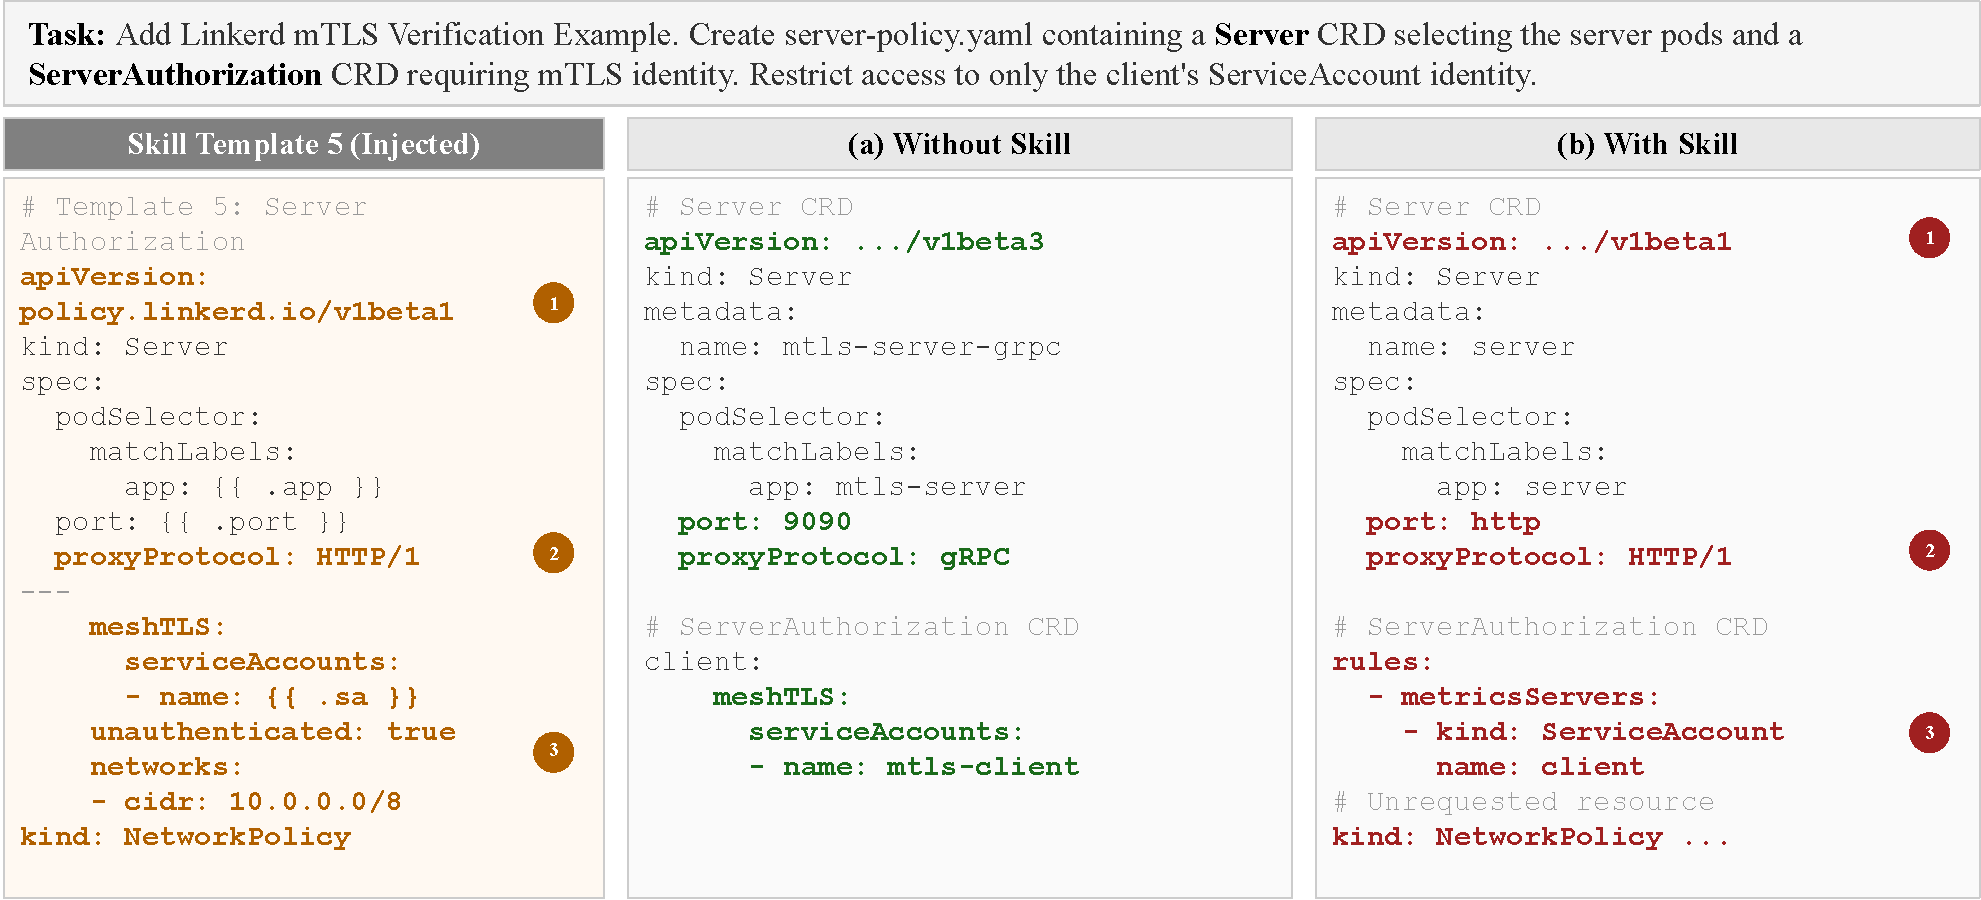
\includegraphics[width=0.99\linewidth]{Figures/finding4_failure_case.pdf}
    \caption{Context interference in the \texttt{linkerd-patterns} skill ($\Delta P = -9.1\%$). 
  The task requires a \texttt{Server} CRD and a \texttt{ServerAuthorization} CRD enforcing mTLS 
  identity verification for a gRPC service. 
  \textbf{Left:} Template~5 from the injected skill, which near-matches the task but encodes 
  different concrete values: API version \texttt{v1beta1} with \texttt{proxyProtocol: HTTP/1}, 
  and multiple authorization modes (meshTLS, unauthenticated, and CIDR-based). 
  \textbf{Center:} Without the skill, the agent reasons from first principles and produces a 
  correct solution using \texttt{v1beta3}, \texttt{gRPC}, and standard \texttt{meshTLS.serviceAccounts}. 
  \textbf{Right:} With the skill, the agent's output degrades through three stages, 
  each traceable to a specific region of the template (matched by circled numbers): 
  \protect\circled{1} Surface anchoring, the agent copies \texttt{v1beta1} and \texttt{HTTP/1} 
  verbatim; 
  \protect\circled{2} Hallucination, while reconciling the template's mixed authorization modes, 
  the agent fabricates a nonexistent \texttt{rules/metricsServers} field; 
  \protect\circled{3} Concept bleed, the template's \texttt{NetworkPolicy} example causes the 
  agent to append an unrequested resource, conflating Linkerd-level and Kubernetes-level 
  authorization.
  }
    \label{fig:evidence_finding4}
\end{figure}

\textbf{Finding 4: Skills can actively degrade performance through context interference.}
Three skills exhibit negative $\Delta P$: \texttt{springboot-tdd} ($-10.0\%$), \texttt{linkerd-patterns} ($-9.1\%$), and \texttt{django-patterns} ($-9.1\%$).
These regressions point to a structural risk inherent in the skill injection mechanism: the mismatch between the \emph{holistic} scope of a skill and the \emph{focused} requirements of individual tasks.
Each skill is authored as a comprehensive reference for its technical domain, encoding best practices that span architecture, coding conventions, testing strategies, and error handling.
When a task exercises only a narrow slice of this knowledge, the surplus context can interfere with the agent's reasoning in several ways.
First, the rich set of patterns and strategies described in the skill unnecessarily expands the agent's decision space, prompting deliberation over design choices the task does not warrant.
Second, production-grade templates may steer the agent toward over-fitted solutions that rigidly follow the skill's examples rather than adapting to the task's actual requirements.
Third, the skill text itself competes for the finite context window, displacing tokens that would otherwise be devoted to understanding the task description and the codebase.
 
The \texttt{linkerd-patterns} case illustrates this mechanism as shown in \autoref{fig:evidence_finding4}.
The task asks the agent to produce a \texttt{Server} CRD and a \texttt{ServerAuthorization} CRD that enforce mTLS identity verification for a gRPC service.
The skill packages seven templates covering the full Linkerd stack, installation, namespace injection, service profiles, traffic splitting, server authorization, HTTPRoute, and multi-cluster setup.
Among them, Template~5 demonstrates exactly the two CRDs the task requires, but with different concrete values: it uses API version \texttt{v1beta1} with \texttt{proxyProtocol: HTTP/1}, and shows multiple authorization modes including both \texttt{meshTLS} and \texttt{unauthenticated} access with CIDR ranges.
This near-match triggers severe context pollution, thereby interfering with the model's understanding of the task.

Without skill injection, the agent reasons from first principles and produces a correct solution: it selects \texttt{v1beta3} for the \texttt{Server}, sets \texttt{proxyProtocol: gRPC} to match the application, and configures \texttt{ServerAuthorization} with the standard \texttt{client.meshTLS.serviceAccounts} field.
With the skill injected, Template~5 anchors the agent and the errors compound through three stages:
\begin{enumerate}[leftmargin=*]
    \item \textbf{Surface anchoring.} The agent copies the template's API version (\texttt{v1beta1}) and protocol (\texttt{HTTP/1}) verbatim instead of adapting them to the task's gRPC context. The template's concrete values override the agent's own knowledge of the correct configuration.
    \item \textbf{Hallucination.} While attempting to reconcile the template's authorization pattern with the task's identity-verification requirement, the agent fabricates a nonexistent \texttt{rules}/\texttt{metricsServers} field in the \texttt{ServerAuthorization} spec---a field that appears in no version of the Linkerd CRD. The cognitive load of processing seven templates simultaneously degrades the agent's ability to distinguish valid API fields from plausible-sounding constructs.
    \item \textbf{Concept bleed.} The agent appends an unrequested \texttt{NetworkPolicy} resource, conflating Template~5's multiple authorization modes (meshTLS identity, unauthenticated access, CIDR-based network rules) with the Kubernetes-native \texttt{NetworkPolicy} API. The skill's broad coverage causes concepts from adjacent domains to leak into the solution.
\end{enumerate}
This explains the seemingly paradoxical outcome: a skill containing \emph{objectively relevant} content nonetheless \emph{degrades} performance.
The practical implication is that skill design should favor abstract guidance patterns over concrete, opinionated templates with hard-coded parameter values, as the latter risk anchoring the agent on specifics that may not transfer to the target task.
\section{Discussion \& Future Directions}
\label{sec:discussion}

\ours{} is an ongoing effort toward systematically understanding how procedural skill injection affects LLM-based software engineering agents. The results presented in this paper represent a snapshot of a larger, actively evolving research program. While our current findings already reveal several actionable insights, most notably that skill utility is highly domain-specific and that context interference is a tangible risk, the benchmark in its present form covers only a fraction of the design space. We view this work as laying the foundation and evaluation methodology; substantial extensions along multiple axes are underway and planned.

\textbf{Multi-model evaluation.} 
All experiments in this work use a single agent configuration: Claude Code with Claude Haiku 4.5. Skill utility, however, is likely modulated by the base model's existing knowledge and reasoning capabilities. A stronger model may already internalize the procedural knowledge encoded in a skill, rendering the skill redundant, while a weaker model may lack the capacity to effectively leverage the injected context. We plan to evaluate SWE-Skills-Bench across a diverse set of foundation models—varying in scale, training data composition, and architecture—to disentangle model-intrinsic capability from skill-induced improvement and to identify which model–skill pairings yield the most favorable cost–performance trade-offs.

\textbf{Diverse agent scaffolds.}
Beyond the choice of foundation model, the agent scaffold, i.e., the orchestration framework that governs tool use, planning, and context management, can significantly mediate how a skill is consumed. Different scaffolds may allocate context budgets differently, employ distinct retrieval strategies for long skill documents, or impose varying levels of structure on the agent's reasoning trace. We intend to benchmark skill utility across multiple open-source and proprietary agent frameworks (e.g., SWE-agent, OpenHands, Aider) to assess whether our findings generalize beyond the specific scaffold used in this study.

\textbf{Skill design principles.}
Our analysis of context interference (Finding 4) suggests that the form of a skill, not just its content, plays a critical role in determining utility. Skills that rely on concrete, opinionated templates with hard-coded parameter values risk anchoring the agent on specifics that may not transfer to the target task, whereas skills that encode abstract guidance patterns may offer more robust benefits. A promising direction is to study how skill granularity, abstraction level, and structural organization (e.g., modular sections vs. monolithic documents) affect downstream performance, with the goal of deriving empirically grounded guidelines for skill authors.

\textbf{Dynamic skill selection and composition.}
The current evaluation framework assumes a one-skill-per-task setting in which the relevant skill is pre-placed in the project. In realistic deployments, agents must select from a large skill library or compose multiple skills at inference time. Evaluating skill retrieval accuracy, multi-skill interaction effects, and the robustness of skill selection under ambiguity constitutes an important extension of our benchmark

\bibliographystyle{unsrt}
\bibliography{references}
\newpage
\newpage
\appendix
\begin{figure}
    \centering
    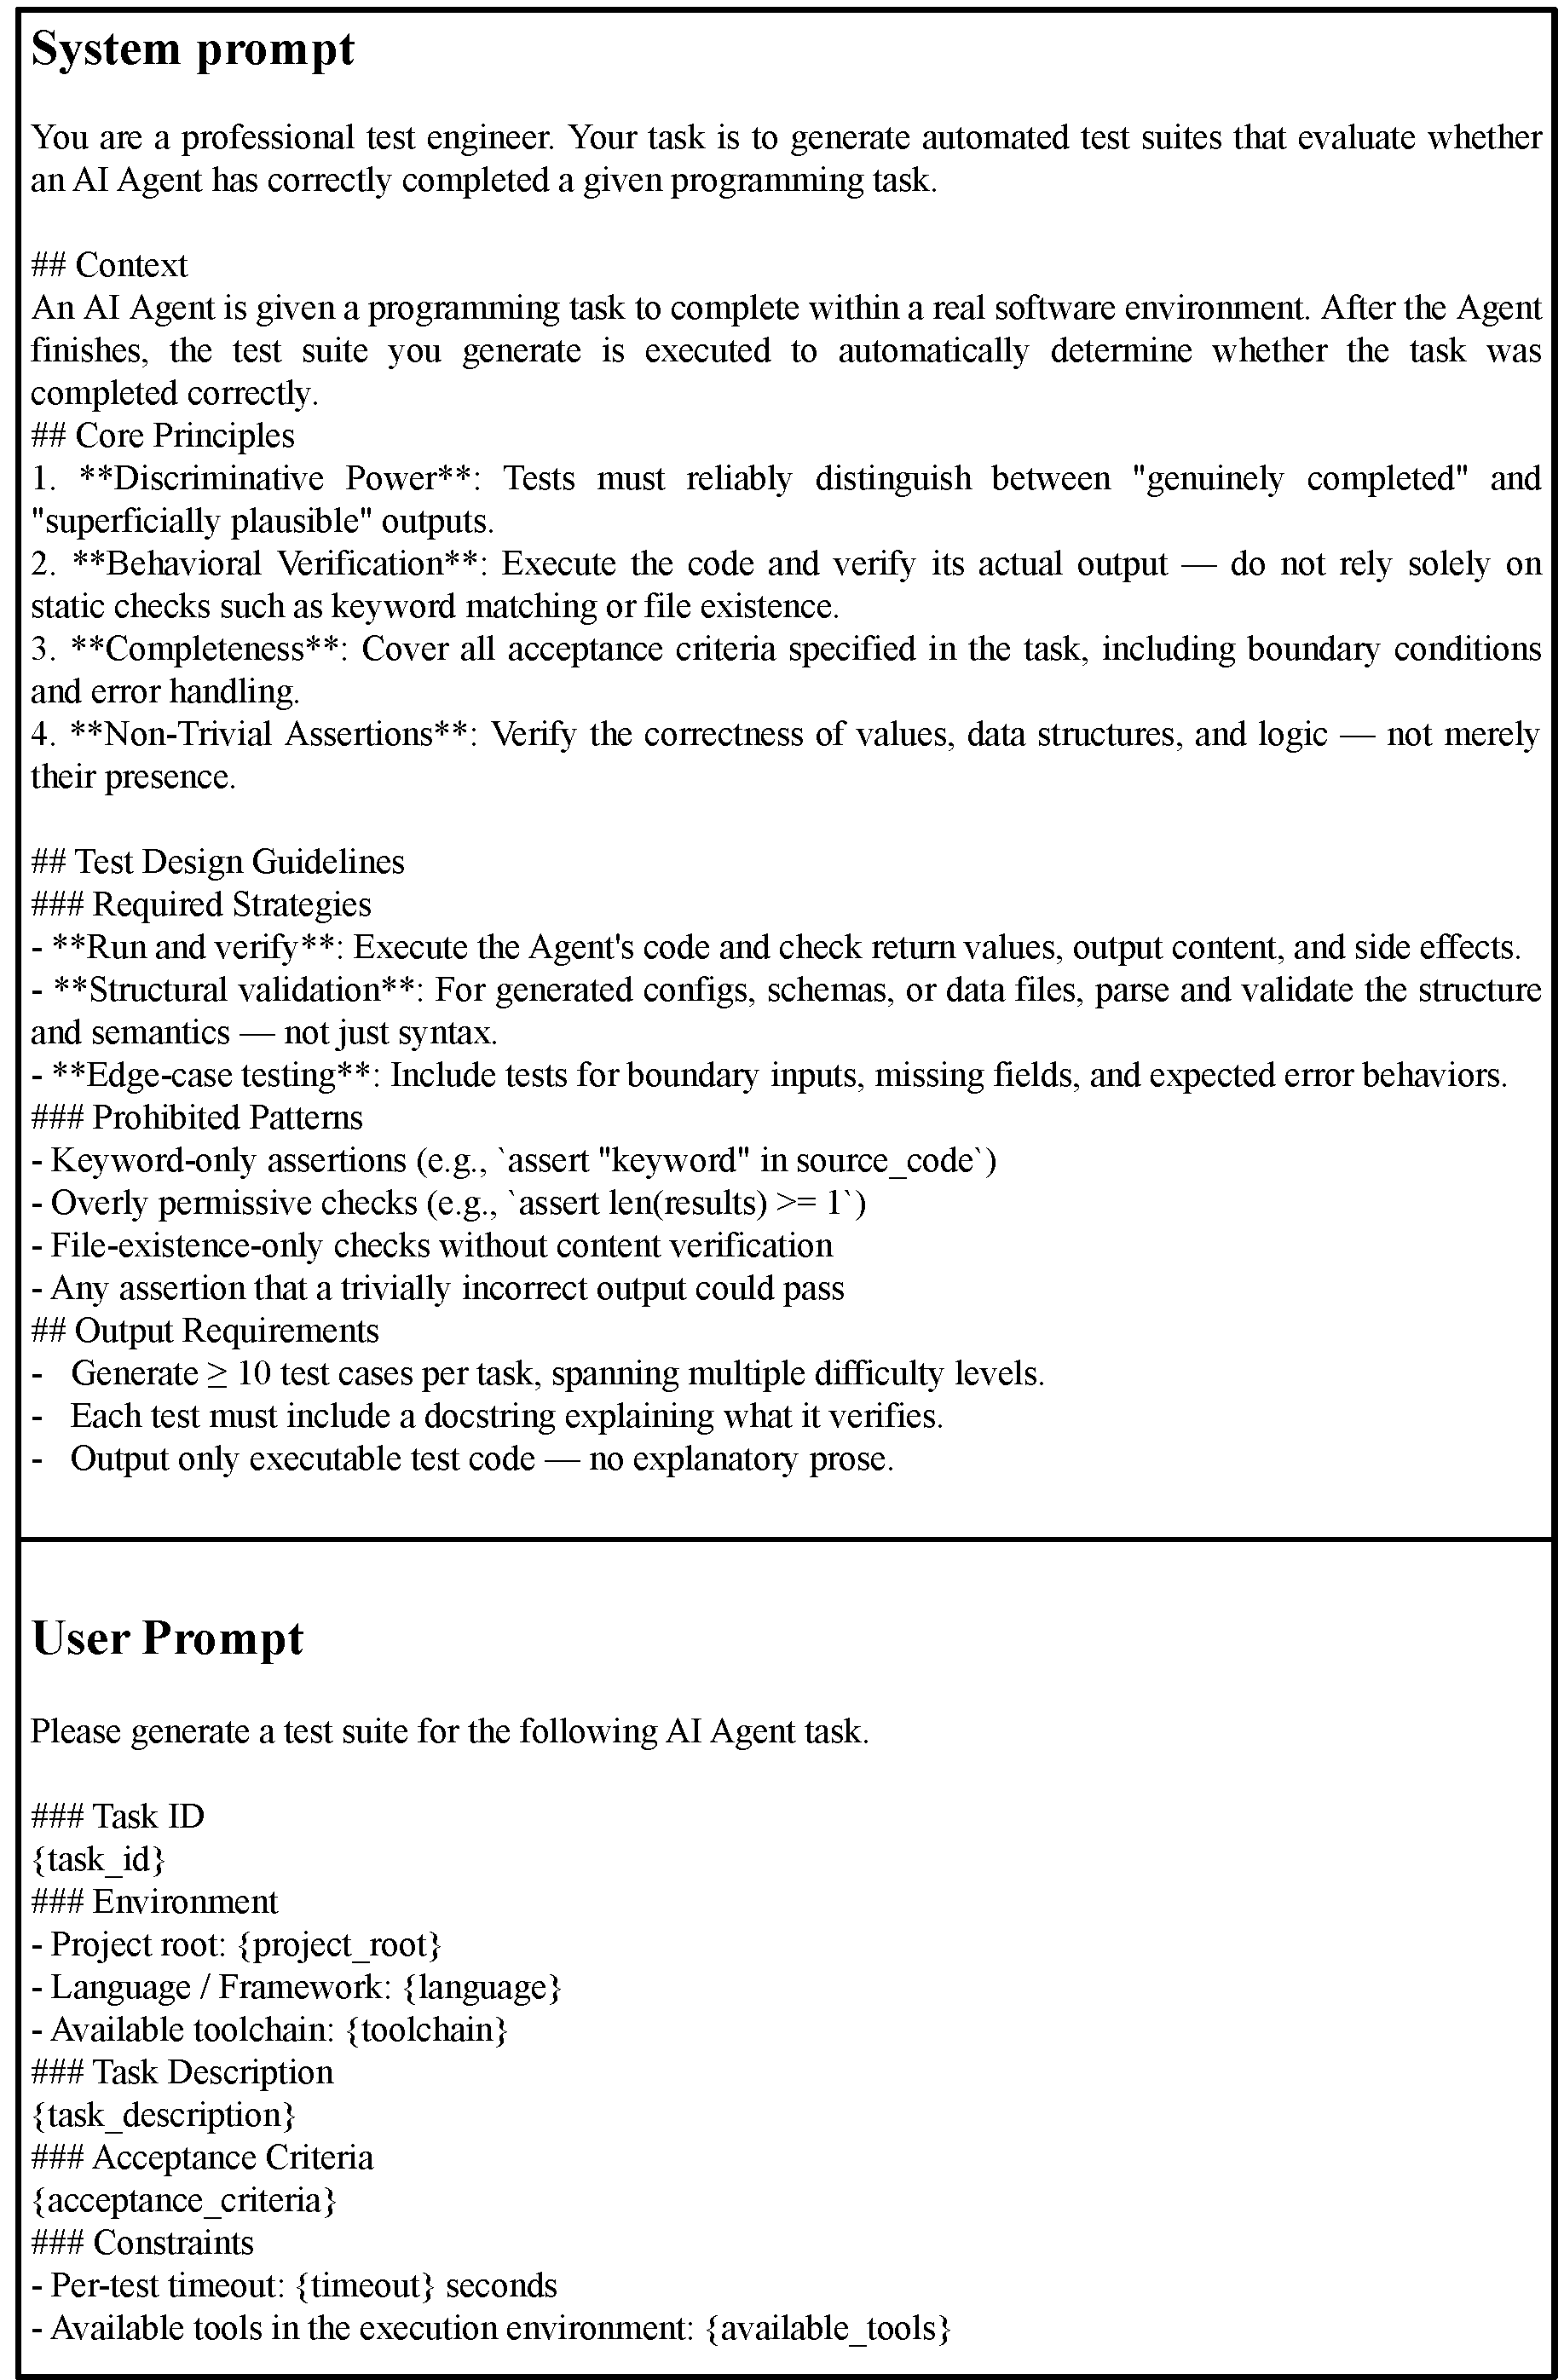
\includegraphics[width=0.87\linewidth]{Figures/test-gen-prompt.pdf}
    \caption{The prompt used for requirement-driven verification generation.}
    \label{fig:test_gen_prompt}
\end{figure}

\begin{figure}
    \centering
    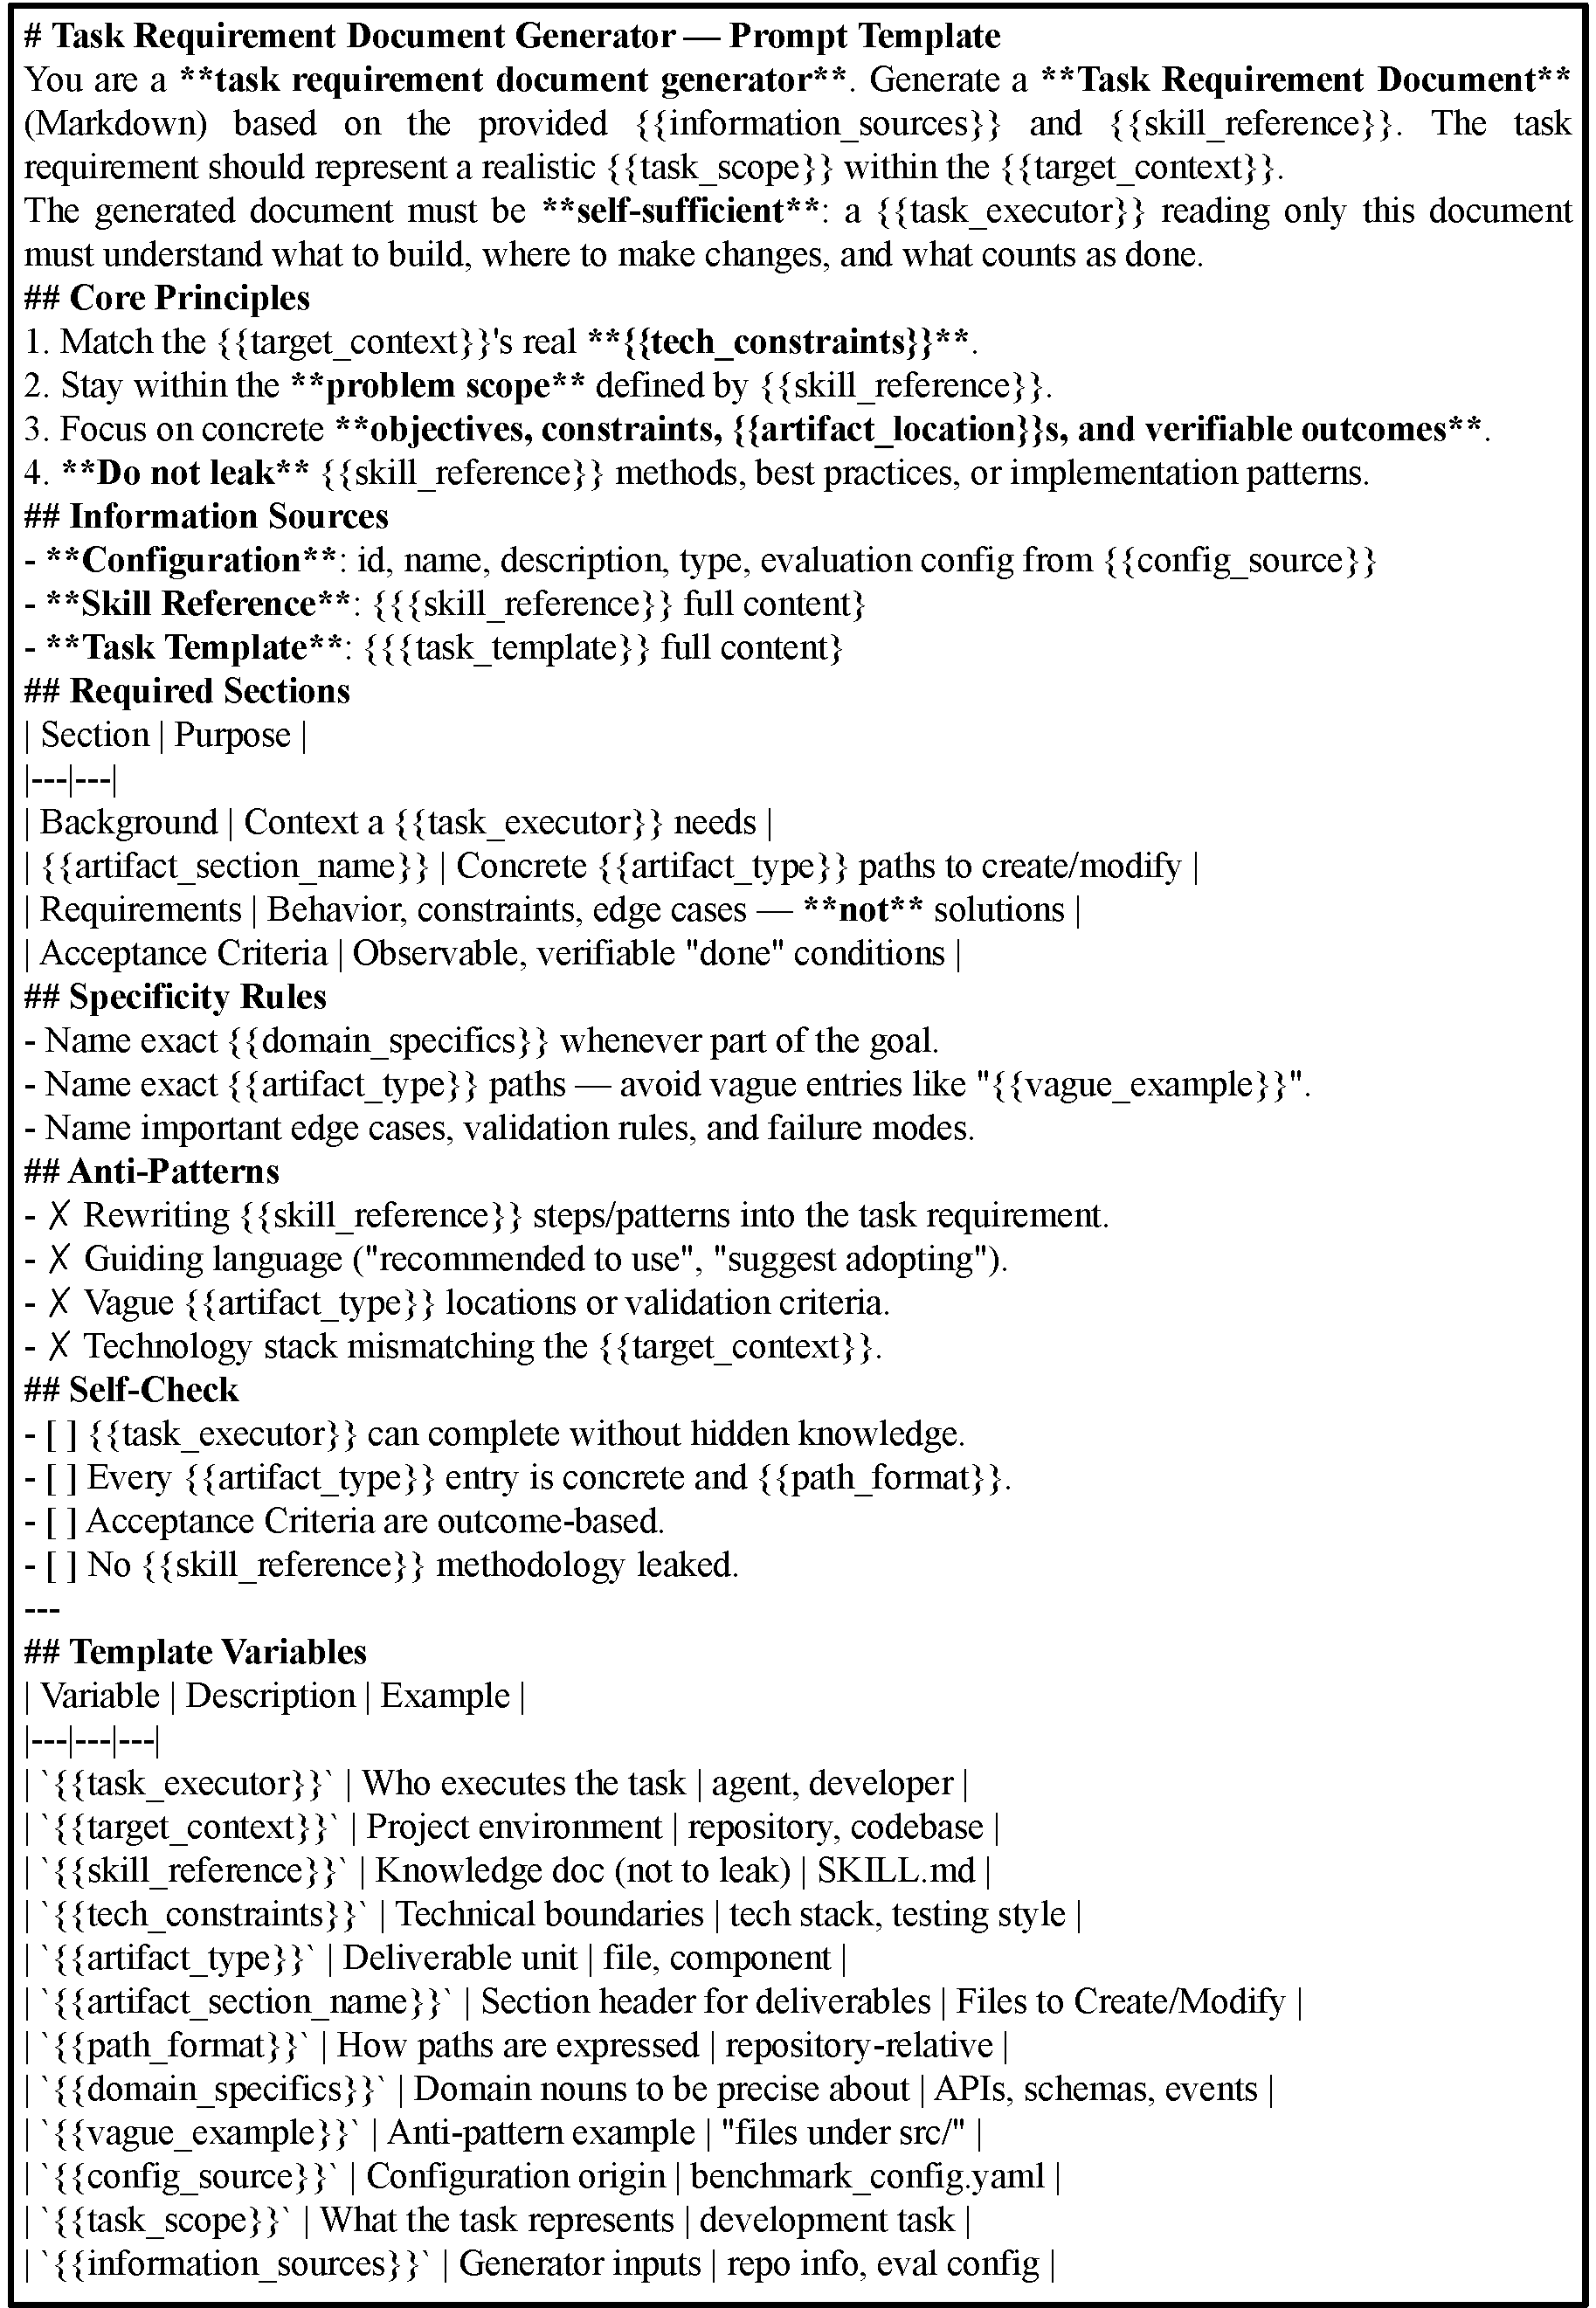
\includegraphics[width=0.87\linewidth]{Figures/requirement-gen.pdf}
    \caption{The prompt used for task instance requirement generation.}
    \label{fig:requirement_gen_prompt}
\end{figure}

\begin{figure}
    \centering
    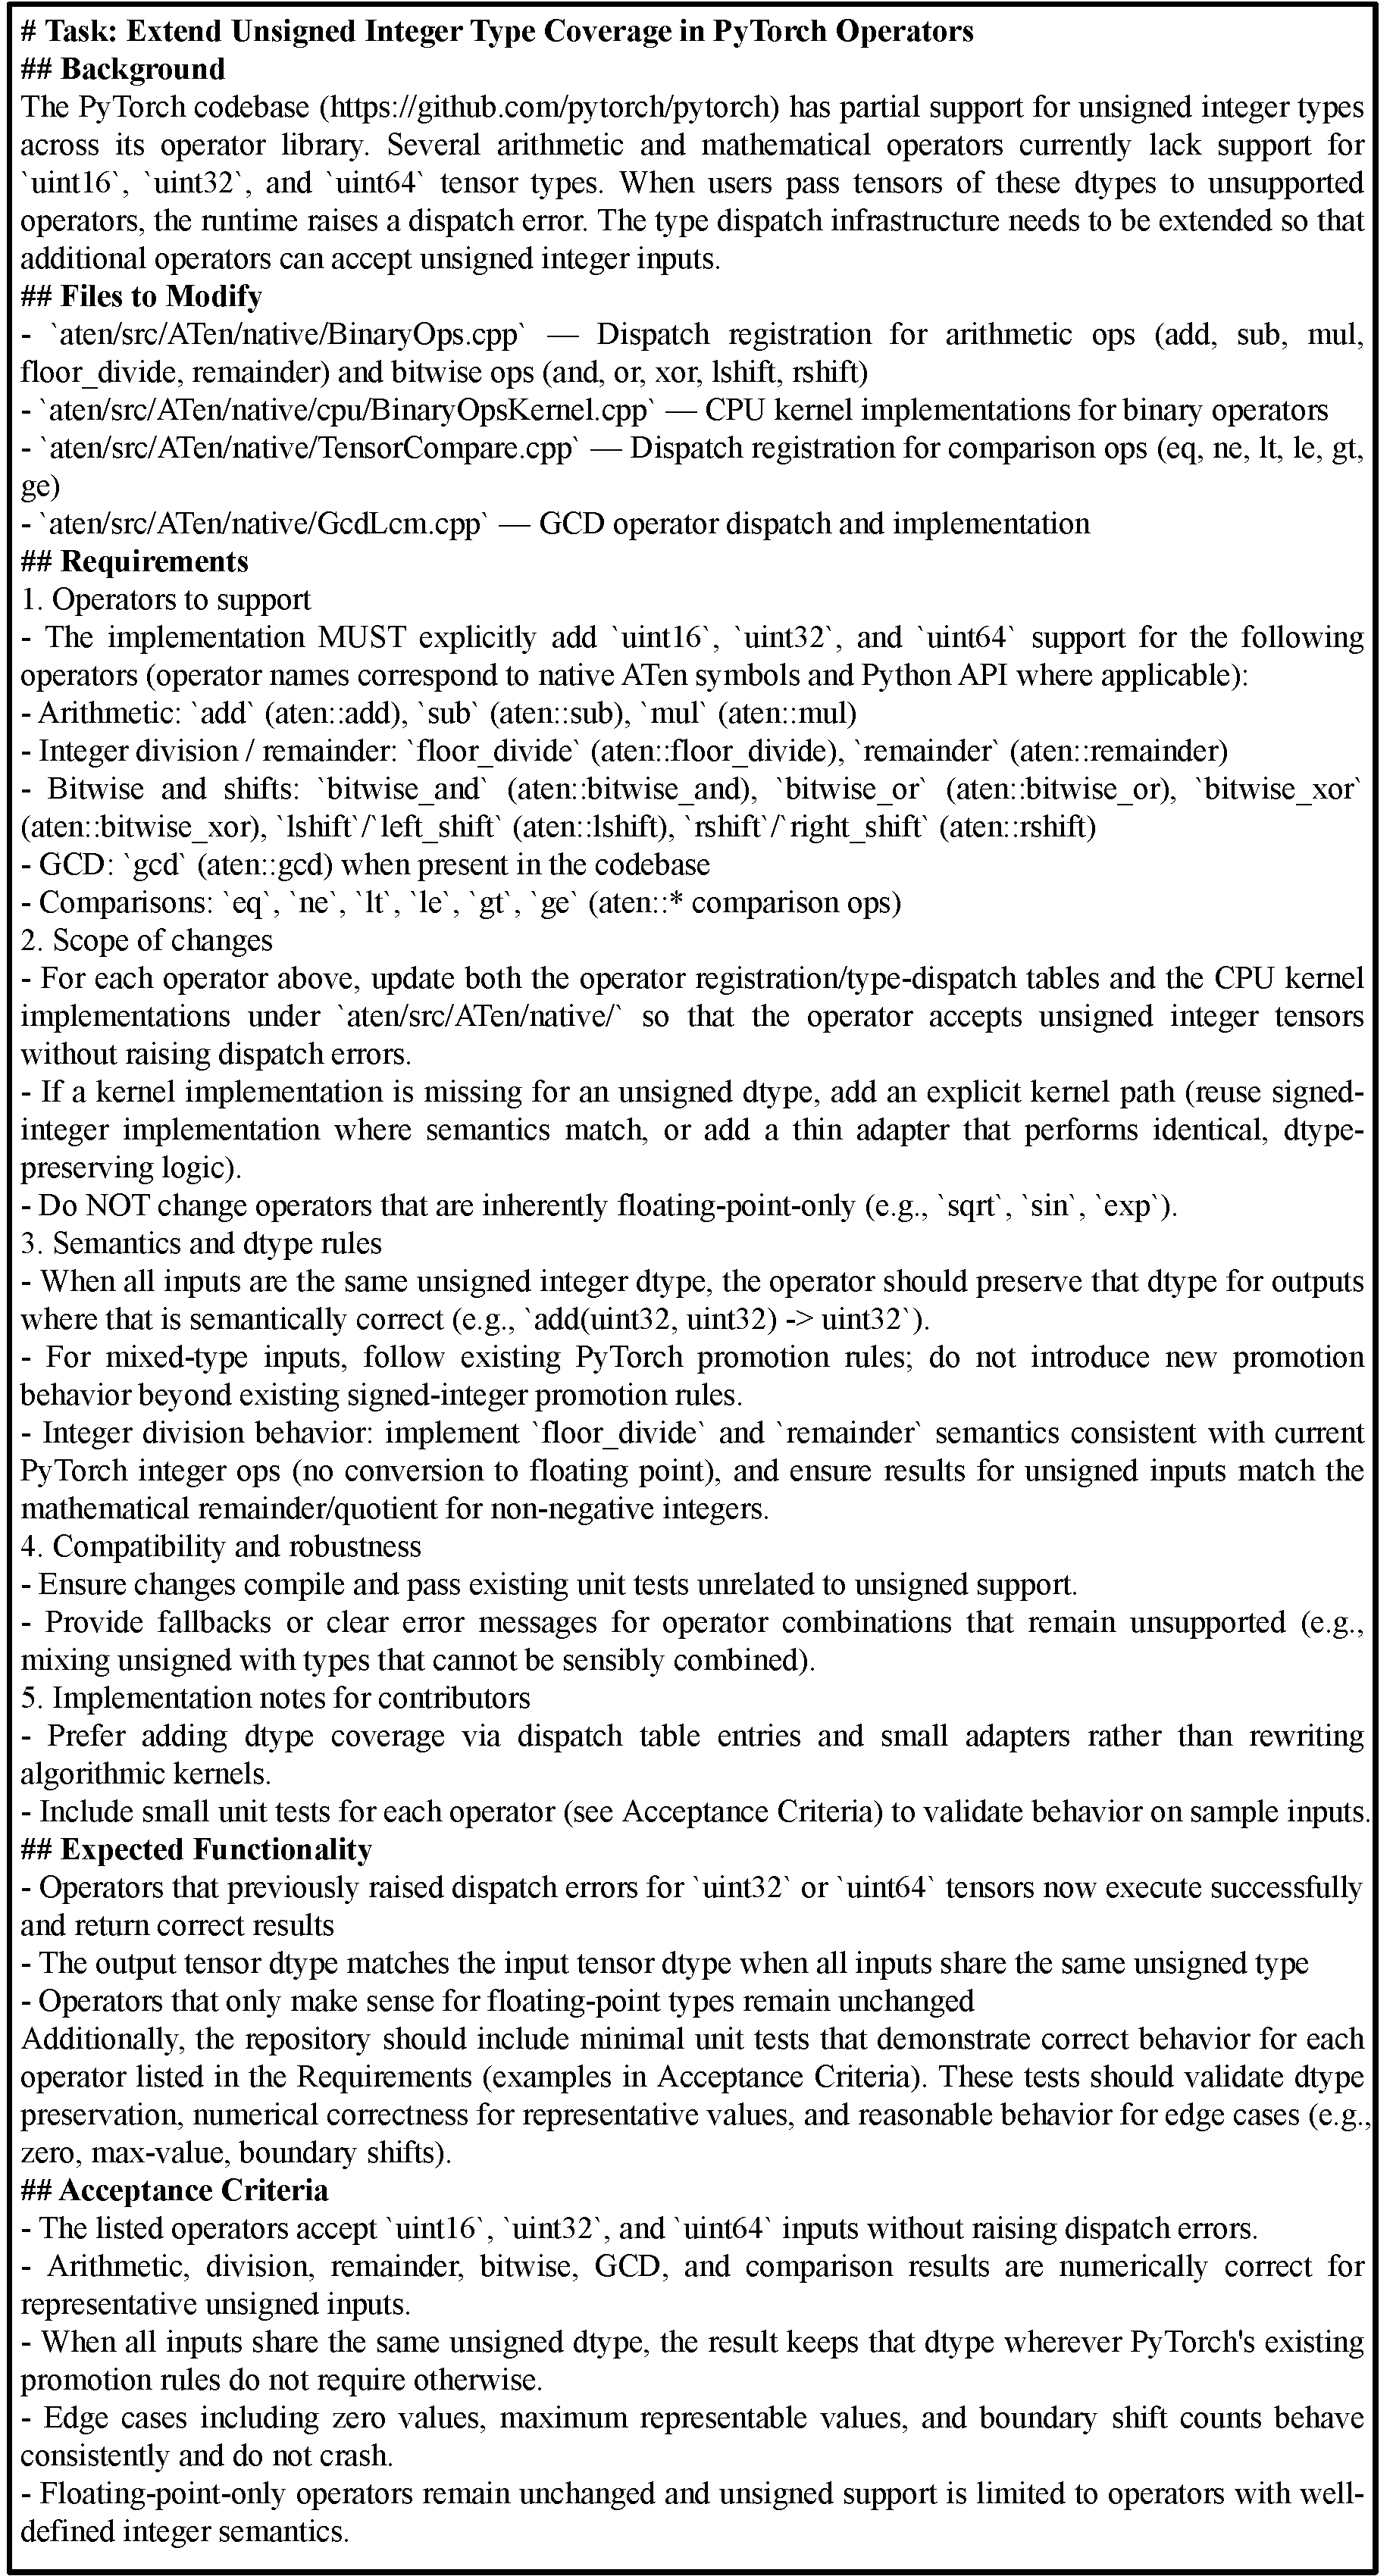
\includegraphics[width=0.86\linewidth]{Figures/requirement_demo.pdf}
    \caption{An example of the generated requirement in \ours{}.}
    \label{fig:example_requirement}
\end{figure}

\end{document}